%%%%%%%%%%%%%%%%%%%%%%%%%%%%%%%%%%%%%%%%%%%%%%%%%%%%%%%%%%%%%%%%%%%%%%%%%%%%%%%%%%%%
%%----------------------------------------------------------------------------------
% DO NOT Change this is the required setting A4 page, 11pt, onside print, book style
%%----------------------------------------------------------------------------------
\documentclass[a4paper,11pt,oneside]{book} 
\usepackage{CS_report} % DO NOT REMOVE THIS LINE. 
%%%%%%%%%%%%%%%%%%%%%%%%%%%%%%%%%%%%%%%%%%%%%%%%%%%%%%%%%%%%%%%%%%%%%%%%%%%%%%%%%%%%


%%%%%%%%%%%%%%%%%%%%%%%%%%%%%%%%%%%%%%%%%%%%%%%%%%%%%%%%%%%%%%%%%%%%%%%%%%%%%%%%%%%%
\begin{document}

    \captionsetup[figure]{margin=1.5cm,font=small,name={Figure},labelsep=colon}
    \captionsetup[table]{margin=1.5cm,font=small,name={Table},labelsep=colon}
    
    \frontmatter
    
    %%%%%%%%%%%%%%%%%%%%%%%%%%%%%%%%%%%%%%%%%%%%%%%%%%%%%%%%%%%%%%%%%%%%%%%%%%%%%%%%
    \begin{titlepage}      
        \begin{center}
            \includegraphics[width=5cm]{figures/logo_ensam.png}\\[0.5cm]
            {\LARGE ENSAM Casablanca\\[0.5cm]
            École Nationale Supérieure D'arts Et Métiers}\\[2cm]
			%{\color{blue} \rule{\textwidth}{1pt}}
			
			% -------------------------------
			% You need to edit some details here
			% -------------------------------  
            \linespread{1.2}\huge {
                %%%%%%%%%%%%%%%%%%%%%%%%%%%%
                %TODO: 1 TITLE of Your PROJECT 
                %%%%%%%%%%%%%%%%%%%%%%%%%%%%
                % change the following line                
                Fake News Detection and Automated Fact Checking Using Machine Learning
            
            }
            \linespread{1}~\\[2cm]
			%{\color{blue} \rule{\textwidth}{1pt}}
            {\Large 
                %%%%%%%%%%%%%%%%%%%%%%%%%%%%
                %TODO: 2 YOUR NAME
                %%%%%%%%%%%%%%%%%%%%%%%%%%%%             
                % change the following line
                Ayoub DYA
                % change end             
            }\\[1cm] 
            

            {\large 
                %%%%%%%%%%%%%%%%%%%%%%%%%%%%
                %TODO: 3 YOUR NAME Supervisor's name(s)
                %%%%%%%%%%%%%%%%%%%%%%%%%%%%             
                % change the following line                
                \emph{Supervisor:} Prof. Badr HIRCHOUA}\\[1cm] % if applicable
            
    		% PLEASE DO NOT CHANGE THIS TEXT %
            \large A report submitted in partial fulfilment of the requirements of\\ENSAM Casablanca\\
            %%%
            %TODO:  verify your degree name
            Artificial Intelligence and Software Engineering 
            \\[0.3cm] 
            \vfill
            
            
            \today % Please update this date you can use \date{April 2020} for fixed date
        \end{center}
    \end{titlepage}
    
    
    % -------------------------------------------------------------------
    % Declaration
    % -------------------------------------------------------------------
    \newpage
    \thispagestyle{empty}
    \chapter*{\Large Declaration}
    % PLEASE CHANGE THIS TEXT EXCEPT YOUR NAME%
    % -------------------------------
    %TODO: PLEASE ONLY UPDATE HERE -- PLEASE WRITE YOUR NAME %    
    % ------------------------------- 
    I,
    %%%%%%%%%%%%%%%%%%%%%%%
     Ayoub DYA, % Madatory part  TODO
    %%%%%%%%%%%%%%%%%%%%%%%
    of ENSAM Casablanca, confirm that this is my own work and figures, tables, equations, code snippets, artworks, and illustrations in this report are original and have not been taken from any other person's work, except where the works of others have been explicitly acknowledged, quoted, and referenced. I understand that if failing to do so will be considered a case of plagiarism. Plagiarism is a form of academic misconduct and will be penalised accordingly. \\
    
    %% Please delete as appropriate. 
    \noindent
    %%%%%%%%%%%%%%%%%%%%%%%%%%%%%%%%%%%%%%%%%%%%%%% 
    %TODO 1 Consent for example copy -  we will use 
    I give consent to a copy of my report being shared with future students as an exemplar. \\
    
    \noindent
    %%%%%%%%%%%%%%%%%%%%%%%%%%%%%%%%%%%%%%%%%%%%%%% 
    %TODO 2 Consent to let the report to use use by library for public use
    I give consent for my work to be made available more widely to members of ENSAM and public with interest in teaching, learning and research. 
    %%%%%%%%%%%%%%%%%%%%%%%%%%%%%%%%%%%%%%%%%%%%%%%
    ~\\[1cm]
    \begin{flushright}
	%------------------------------ 
	% change the following line
    %TODO: PLEASE UPDATE  Your Name  -------------------------------%
	Ayoub DYA % Please change it to your name
    
    \today
    \end{flushright}

     
    % -------------------------------------------------------------------
    % Abstract and Acknowledgement
    % -------------------------------------------------------------------
    
    %Two resources useful for abstract writing.
% Guidance of how to write an abstract/summary provided by Nature: https://cbs.umn.edu/sites/cbs.umn.edu/files/public/downloads/Annotated_Nature_abstract.pdf %https://writingcenter.gmu.edu/guides/writing-an-abstract
\chapter*{\center \Large  Abstract}

The spread of fake news on social media and online platforms has become a major problem in today's digital world. False information can influence public opinion, affect elections, and cause harm to individuals and society. This project presents UnFake, an AI-powered fake news detection system that uses machine learning to classify news content as either ``Fake'' or ``Real.''

The system uses two different machine learning models to handle different types of content. For short statements and headlines, a fine-tuned RoBERTa transformer model is used, which achieves an accuracy of 74.69\% and an F1 score of 75.02\% on the test set. For longer articles, a Gradient Boosting Classifier combined with TF-IDF vectorization is used, achieving an impressive accuracy of 99.57\%. The dual-model approach allows the system to handle both short claims and full news articles effectively.

The project includes a complete web application with a FastAPI backend and a modern frontend interface. Users can input statements or articles through the web interface and receive instant predictions with confidence scores. The system was trained on multiple datasets including PolitiFact fact-checked statements and news article datasets containing over 44,000 articles.

The results show that machine learning can be an effective tool for detecting fake news, especially for longer articles where the model achieves near-perfect accuracy. The headline model shows more modest performance, reflecting the challenge of classifying short statements with limited context. Future work could focus on improving the headline model's accuracy and adding support for multiple languages.

~\\[1cm]
\noindent
\textbf{Keywords:} fake news detection, machine learning, natural language processing, RoBERTa, gradient boosting

\vfill
\noindent
\newline
\noindent
\textbf{GitHub Repository:} \url{https://github.com/ayoubdya/unfake}


    % -------------------------------------------------------------------
	% Acknowledgement
	% -------------------------------------------------------------------
   
    \chapter*{\center \Large  Acknowledgements}

I would like to thank my supervisor Prof. Badr HIRCHOUA for his guidance throughout this project, ENSAM Casablanca for providing the necessary resources, and the open-source community for developing the tools that made this work possible. Special thanks to my family and friends for their support.  

   
    
    % -------------------------------------------------------------------
    % Contents, list of figures, list of tables
    % -------------------------------------------------------------------
    
    \tableofcontents
    \listoffigures
    \listoftables
    \chapter*{List of Abbreviations}
\chaptermark{List of Abbreviations}
%%%%%%%%%%%%%%%%%%%%%%%%%%%%%%%%%%%
%%  Abbreviations for UnFake Fake News Detection Project
%%%%%%%%%%%%%%%%%%%%%%%%%%%%%%%%%%%
\begin{abbrv}
    
    \item[AI]               Artificial Intelligence
    \item[API]              Application Programming Interface
    \item[ASGI]             Asynchronous Server Gateway Interface
    \item[BERT]             Bidirectional Encoder Representations from Transformers
    \item[CORS]             Cross-Origin Resource Sharing
    \item[CPU]              Central Processing Unit
    \item[CSS]              Cascading Style Sheets
    \item[CSV]              Comma-Separated Values
    \item[CUDA]             Compute Unified Device Architecture
    \item[DOM]              Document Object Model
    \item[F1]               F1 Score (harmonic mean of precision and recall)
    \item[GPU]              Graphics Processing Unit
    \item[HTML]             HyperText Markup Language
    \item[HTTP]             HyperText Transfer Protocol
    \item[JSON]             JavaScript Object Notation
    \item[ML]               Machine Learning
    \item[MLM]              Masked Language Modeling
    \item[NLP]              Natural Language Processing
    \item[NLTK]             Natural Language Toolkit
    \item[REST]             Representational State Transfer
    \item[RoBERTa]          Robustly Optimized BERT Pre-training Approach
    \item[ROC-AUC]          Receiver Operating Characteristic - Area Under Curve
    \item[TF-IDF]           Term Frequency - Inverse Document Frequency
    \item[UI]               User Interface
    \item[URL]              Uniform Resource Locator
    
\end{abbrv}
 %  Enter your list of Abbreviation and Symbols in this file



    
    
    %%%%%%%%%%%%%%%%%%%%%%%%%%%%%%%%%%%%%%%%%%%%%%%%%%%%%%%%%%%%%%%%%%%%%%%%
    %%                                                                    %%  
    %%  Main chapters and sections of your project                        %%  
    %%  Everything from here on needs updates in your own words and works %%
    %%                                                                    %%
    %%%%%%%%%%%%%%%%%%%%%%%%%%%%%%%%%%%%%%%%%%%%%%%%%%%%%%%%%%%%%%%%%%%%%%%%
    \mainmatter
    % Read for preparation of document in LaTex 
    % Lamport, L. (1986), LATEX: A Document Preparation System, Addison-Wesley.
    
    \chapter{Introduction}
\label{ch:into}

In today's digital age, the spread of false information has become one of the most pressing challenges facing society. Fake news, which refers to intentionally misleading or false information presented as legitimate news, spreads rapidly through social media platforms and online news sources. This misinformation can have serious consequences, from influencing election outcomes to causing public health crises. The need for automated tools to detect and flag fake news has never been more important.

This project presents UnFake, an AI-powered fake news detection system that uses machine learning to classify news content as either ``Fake'' or ``Real.'' The system combines modern deep learning techniques with traditional machine learning approaches to provide accurate predictions for both short statements and full-length articles.

%%%%%%%%%%%%%%%%%%%%%%%%%%%%%%%%%%%%%%%%%%%%%%%%%%%%%%%%%%%%%%%%%%%%%%%%%%%%%%%%%%%
\section{Background}
\label{sec:into_back}

The term ``fake news'' gained widespread attention during the 2016 United States presidential election, when false stories spread rapidly on social media platforms. However, the problem of misinformation is not new. What has changed is the speed and scale at which false information can now spread through digital channels.

Social media platforms like Facebook, Twitter, and WhatsApp have made it easy for anyone to share content with millions of people instantly. While this has many benefits for communication and access to information, it also creates opportunities for bad actors to spread false information. Studies have shown that fake news spreads faster than true news on social media, partly because false stories are often more sensational and emotionally engaging.

The consequences of fake news can be severe. During the COVID-19 pandemic, misinformation about treatments and vaccines contributed to public health problems. In politics, fake news has been used to manipulate public opinion and undermine trust in democratic institutions. In financial markets, false information can cause stock prices to swing wildly, affecting investors and companies alike.

Traditional fact-checking by journalists is effective but slow and cannot keep up with the volume of content produced online. This has created a need for automated systems that can quickly analyze news content and flag potentially false information for human review.

Machine learning offers a promising approach to this problem. By training models on large datasets of verified true and false news, these systems can learn patterns that distinguish real news from fake news. Natural Language Processing (NLP) techniques allow these models to understand the content of text and make predictions based on linguistic features, writing style, and other characteristics.

%%%%%%%%%%%%%%%%%%%%%%%%%%%%%%%%%%%%%%%%%%%%%%%%%%%%%%%%%%%%%%%%%%%%%%%%%%%%%%%%%%%
\section{Problem Statement}
\label{sec:intro_prob_art}

The main problem addressed by this project is: \textbf{How can we automatically classify news content as real or fake using machine learning techniques?}

This problem involves several challenges:

\begin{enumerate}
    \item \textbf{Different content types:} News appears in different formats, from short headlines and social media posts to full-length articles. A system needs to handle both types effectively.
    
    \item \textbf{Evolving tactics:} Creators of fake news constantly adapt their methods to avoid detection, meaning models may need regular updates to remain effective.
    
    \item \textbf{Context dependence:} The same statement might be true in one context and false in another, making classification challenging.
    
    \item \textbf{Bias in training data:} Datasets used for training may contain biases that could affect model performance.
    
    \item \textbf{User accessibility:} The system should be easy to use for non-technical users who want to verify news content.
\end{enumerate}

%%%%%%%%%%%%%%%%%%%%%%%%%%%%%%%%%%%%%%%%%%%%%%%%%%%%%%%%%%%%%%%%%%%%%%%%%%%%%%%%%%%
\section{Aims and Objectives}
\label{sec:intro_aims_obj}

\subsection{Aim}
The aim of this project is to develop a complete fake news detection system that can accurately classify news content as real or fake, and provide this functionality through an easy-to-use web interface.

\subsection{Objectives}
To achieve this aim, the following objectives were set:

\begin{enumerate}
    \item \textbf{Data collection and preparation:} Gather and preprocess datasets containing labeled examples of real and fake news for model training.
    
    \item \textbf{Headline model development:} Train a deep learning model using transformer architecture (RoBERTa) to classify short statements and headlines.
    
    \item \textbf{Article model development:} Train a traditional machine learning model (Gradient Boosting) to classify full-length news articles.
    
    \item \textbf{API development:} Create a REST API using FastAPI to serve model predictions to client applications.
    
    \item \textbf{Frontend development:} Build a user-friendly web interface that allows users to input text and receive classification results.
    
    \item \textbf{System integration:} Integrate all components into a complete, working system.
    
    \item \textbf{Evaluation:} Evaluate model performance using appropriate metrics such as accuracy, precision, recall, and F1 score.
\end{enumerate}

%%%%%%%%%%%%%%%%%%%%%%%%%%%%%%%%%%%%%%%%%%%%%%%%%%%%%%%%%%%%%%%%%%%%%%%%%%%%%%%%%%%
\section{Solution Approach}
\label{sec:intro_sol}

The solution uses a dual-model approach to handle different types of content effectively:

\subsection{Headline Model}
\label{sec:intro_headline_model}
For short statements and headlines, a fine-tuned RoBERTa (Robustly Optimized BERT Pretraining Approach) transformer model is used. RoBERTa is a variant of BERT that has been trained on a larger dataset with improved training methodology. The model was fine-tuned on a dataset of fact-checked statements from PolitiFact, a respected fact-checking organization. This approach leverages the power of transfer learning, where a model pre-trained on a large corpus of text is adapted for a specific task.

\subsection{Article Model}
\label{sec:intro_article_model}
For full-length articles, a Gradient Boosting Classifier combined with TF-IDF (Term Frequency-Inverse Document Frequency) vectorization is used. This traditional machine learning approach works well for longer texts where the bag-of-words representation can capture important patterns. The model was trained on a dataset of over 44,000 news articles labeled as real or fake.

\subsection{System Architecture}
\label{sec:intro_architecture}
The complete system follows a three-tier architecture:
\begin{itemize}
    \item \textbf{Frontend:} A web application built with HTML, CSS, and JavaScript that provides the user interface.
    \item \textbf{Backend:} A FastAPI application that handles requests, preprocesses text, and runs model inference.
    \item \textbf{Models:} The trained machine learning models stored as files and loaded into memory at startup.
\end{itemize}

%%%%%%%%%%%%%%%%%%%%%%%%%%%%%%%%%%%%%%%%%%%%%%%%%%%%%%%%%%%%%%%%%%%%%%%%%%%%%%%%%%%
\section{Summary of Contributions and Achievements}
\label{sec:intro_sum_results}

The main contributions and achievements of this project are:

\begin{enumerate}
    \item \textbf{Dual-model system:} Development of a system that uses two different models optimized for different content types, achieving 74.69\% accuracy on headlines and 99.57\% accuracy on articles.
    
    \item \textbf{Complete web application:} Implementation of a full-stack web application with an intuitive user interface for analyzing news content.
    
    \item \textbf{REST API:} Creation of a well-documented API that can be used by other applications to access the fake news detection functionality.
    
    \item \textbf{Data pipeline:} Development of data collection tools, including a web scraper for PolitiFact to gather fact-checked statements.
    
    \item \textbf{Comprehensive evaluation:} Thorough evaluation of model performance with detailed metrics and analysis.
\end{enumerate}

%%%%%%%%%%%%%%%%%%%%%%%%%%%%%%%%%%%%%%%%%%%%%%%%%%%%%%%%%%%%%%%%%%%%%%%%%%%%%%%%%%%
\section{Organization of the Report}
\label{sec:intro_org}

This report is organized into seven chapters:

\begin{itemize}
    \item \textbf{Chapter~\ref{ch:into} (Introduction):} Provides background information, problem statement, aims and objectives, and an overview of the solution approach.
    
    \item \textbf{Chapter~\ref{ch:lit_rev} (Literature Review):} Reviews existing research on fake news detection, natural language processing, and machine learning techniques relevant to this project.
    
    \item \textbf{Chapter~\ref{ch:method} (Methodology):} Describes the datasets used, the machine learning models developed, and the system architecture in detail.
    
    \item \textbf{Chapter~\ref{ch:results} (Results):} Presents the performance of the trained models and demonstrates the working system.
    
    \item \textbf{Chapter~\ref{ch:evaluation} (Discussion and Analysis):} Analyzes the results, discusses their significance, and examines the limitations of the approach.
    
    \item \textbf{Chapter~\ref{ch:con} (Conclusions and Future Work):} Summarizes the project findings and suggests directions for future development.
    
    \item \textbf{Chapter~\ref{ch:reflection} (Reflection):} Reflects on the learning experience and challenges encountered during the project.
\end{itemize}


    \chapter{Literature Review}
\label{ch:lit_rev}

This chapter reviews existing research and technologies related to fake news detection, natural language processing, and the machine learning techniques used in this project. Understanding the current state of the field helps to position the UnFake system within the broader context of fake news detection research.

\section{Understanding Fake News}
\label{sec:understanding_fake_news}

Fake news can be defined as intentionally false or misleading information presented as legitimate news. However, the term covers a spectrum of different types of misinformation~\citep{shu2017fake}:

\begin{itemize}
    \item \textbf{Satire and parody:} Content that is not intended to cause harm but uses humor and exaggeration. This is usually clearly labeled as satire.
    
    \item \textbf{Misleading content:} Information that uses misleading framing of issues or individuals.
    
    \item \textbf{Imposter content:} Content that impersonates genuine news sources.
    
    \item \textbf{Fabricated content:} Completely false content designed to deceive.
    
    \item \textbf{False context:} Genuine content shared with false contextual information.
    
    \item \textbf{Manipulated content:} Genuine information or imagery that has been altered to deceive.
\end{itemize}

The spread of fake news is driven by several factors. Social media algorithms often prioritize engaging content, which tends to be sensational and emotionally provocative. People are more likely to share content that aligns with their existing beliefs, a phenomenon known as confirmation bias. Additionally, the speed of online communication means that false information can spread widely before fact-checkers have time to verify it.

\section{Natural Language Processing for Text Classification}
\label{sec:nlp_text_classification}

Natural Language Processing (NLP) is a field of artificial intelligence that focuses on enabling computers to understand and process human language. Text classification is a fundamental NLP task where the goal is to assign predefined categories to text documents.

\subsection{Traditional Approaches}
\label{subsec:traditional_approaches}

Traditional text classification approaches typically involve two main steps: feature extraction and classification.

\textbf{Feature extraction} converts text into numerical representations that machine learning algorithms can process. Common techniques include:

\begin{itemize}
    \item \textbf{Bag of Words (BoW):} Represents text as a collection of word counts, ignoring grammar and word order.
    
    \item \textbf{TF-IDF (Term Frequency-Inverse Document Frequency):} Weights words by how important they are to a document relative to the entire corpus. Words that appear frequently in a document but rarely in others receive higher weights.
    
    \item \textbf{N-grams:} Captures sequences of n consecutive words, preserving some word order information.
\end{itemize}

\textbf{Classification algorithms} commonly used for text classification include:

\begin{itemize}
    \item \textbf{Naive Bayes:} A probabilistic classifier based on Bayes' theorem, assuming independence between features.
    
    \item \textbf{Support Vector Machines (SVM):} Finds the optimal hyperplane that separates different classes in the feature space.
    
    \item \textbf{Random Forest:} An ensemble method that builds multiple decision trees and combines their predictions.
    
    \item \textbf{Gradient Boosting:} An ensemble technique that builds trees sequentially, with each tree correcting the errors of the previous ones. This approach is used in the UnFake article model.
\end{itemize}

\subsection{Deep Learning Approaches}
\label{subsec:deep_learning_approaches}

Deep learning has revolutionized NLP in recent years. Key developments include:

\textbf{Word embeddings} such as Word2Vec and GloVe represent words as dense vectors where semantically similar words are close together in the vector space.

\textbf{Recurrent Neural Networks (RNNs)} and their variants (LSTM, GRU) can process sequences of text, maintaining memory of previous words in the sequence.

\textbf{Transformer architecture}, introduced in the paper ``Attention Is All You Need''~\citep{vaswani2017attention}, uses self-attention mechanisms to process entire sequences in parallel, leading to significant improvements in NLP tasks.

\textbf{Pre-trained language models} like BERT (Bidirectional Encoder Representations from Transformers)~\citep{devlin2019bert} and its variants have achieved state-of-the-art results on many NLP benchmarks. These models are pre-trained on large text corpora and can be fine-tuned for specific tasks with relatively small amounts of labeled data.

\section{Transformer Models and RoBERTa}
\label{sec:transformers_roberta}

The transformer architecture has become the foundation for modern NLP. Unlike RNNs, transformers process all positions in a sequence simultaneously using attention mechanisms. This allows them to capture long-range dependencies in text more effectively.

BERT (Bidirectional Encoder Representations from Transformers) was a breakthrough in NLP~\citep{devlin2019bert}. It uses bidirectional training, meaning it considers context from both directions (left and right) when understanding a word. BERT is pre-trained on two tasks: masked language modeling (predicting masked words) and next sentence prediction.

RoBERTa (Robustly Optimized BERT Pretraining Approach)~\citep{liu2019roberta} improves on BERT in several ways:

\begin{itemize}
    \item Training on more data for longer periods
    \item Removing the next sentence prediction task
    \item Using longer sequences during training
    \item Dynamically changing the masking pattern during training
\end{itemize}

These modifications result in better performance on many downstream tasks. RoBERTa is particularly effective for text classification tasks, making it a good choice for the headline model in UnFake.

\section{Existing Fake News Detection Systems}
\label{sec:existing_systems}

Several approaches to automated fake news detection have been developed:

\subsection{Content-Based Methods}
\label{subsec:content_based}

Content-based methods analyze the text of news articles to detect fake news. Features that have been found useful include:

\begin{itemize}
    \item Writing style and quality
    \item Sentiment and emotional language
    \item Use of sensational or exaggerated claims
    \item Presence of specific linguistic patterns
\end{itemize}

Research has shown that fake news often uses more emotional and sensational language than real news. The writing style may also be different, with fake news sometimes having lower grammatical quality.

\subsection{Social Context Methods}
\label{subsec:social_context}

Social context methods examine how content spreads on social networks. Features include:

\begin{itemize}
    \item User profiles and credibility
    \item Sharing patterns and network structure
    \item User engagement and reactions
    \item Propagation speed and patterns
\end{itemize}

These methods can be effective because fake news often spreads differently than real news, with different user engagement patterns.

\subsection{Knowledge-Based Methods}
\label{subsec:knowledge_based}

Knowledge-based methods compare claims against verified knowledge bases or fact-checking databases. These approaches can be highly accurate but are limited to claims for which verified information exists.

\section{Gradient Boosting for Classification}
\label{sec:gradient_boosting}

Gradient Boosting is an ensemble learning method that combines multiple weak learners (typically decision trees) to create a strong classifier. The key ideas are:

\begin{enumerate}
    \item Start with an initial prediction (often the mean for regression or log-odds for classification)
    \item Calculate the residuals (errors) of the current model
    \item Fit a new tree to predict these residuals
    \item Add the new tree's predictions to the model (scaled by a learning rate)
    \item Repeat steps 2-4 for a specified number of iterations
\end{enumerate}

The ``gradient'' in gradient boosting refers to the use of gradient descent optimization to minimize a loss function. Each new tree is fit to the negative gradient of the loss function with respect to the current predictions.

Gradient Boosting works well for many classification tasks, including text classification with TF-IDF features. It is particularly effective when:

\begin{itemize}
    \item The relationship between features and target is complex
    \item Feature interactions are important
    \item The dataset is not too large (deep learning may be better for very large datasets)
\end{itemize}

For the UnFake article model, Gradient Boosting combined with TF-IDF achieves excellent performance, demonstrating that traditional machine learning methods remain competitive for certain tasks.

\section{Summary}
\label{sec:lit_summary}

This literature review has covered the key concepts and technologies relevant to the UnFake fake news detection system:

\begin{itemize}
    \item Fake news is a complex problem with various types of misinformation
    \item NLP techniques, from traditional TF-IDF to modern transformers, enable machines to understand and classify text
    \item Transformer models like RoBERTa have achieved state-of-the-art results in text classification
    \item Multiple approaches exist for fake news detection, including content-based, social context, and knowledge-based methods
    \item Gradient Boosting is an effective traditional machine learning method for text classification
\end{itemize}

The UnFake system combines modern deep learning (RoBERTa for headlines) with traditional machine learning (Gradient Boosting for articles) to provide a comprehensive solution for fake news detection.
 % https://guides.library.bloomu.edu/litreview
    \chapter{Methodology}
\label{ch:method}

This chapter describes the methodology used to develop the UnFake fake news detection system. It covers the datasets used for training, the machine learning models developed, the system architecture, and the implementation details.

\section{System Overview}
\label{sec:system_overview}

The UnFake system uses a dual-model approach to classify news content as real or fake. Two separate models are used to handle different types of content:

\begin{enumerate}
    \item \textbf{Headline Model:} A fine-tuned RoBERTa transformer for classifying short statements and headlines (up to 256 tokens).
    
    \item \textbf{Article Model:} A Gradient Boosting Classifier with TF-IDF vectorization for classifying full-length news articles.
\end{enumerate}

This approach allows the system to optimize performance for each content type. Short statements require a model that can understand context from limited text, while longer articles provide more features for traditional machine learning approaches.

Figure~\ref{fig:system_architecture} shows the overall system architecture.

\begin{figure}[!ht]
    \centering
    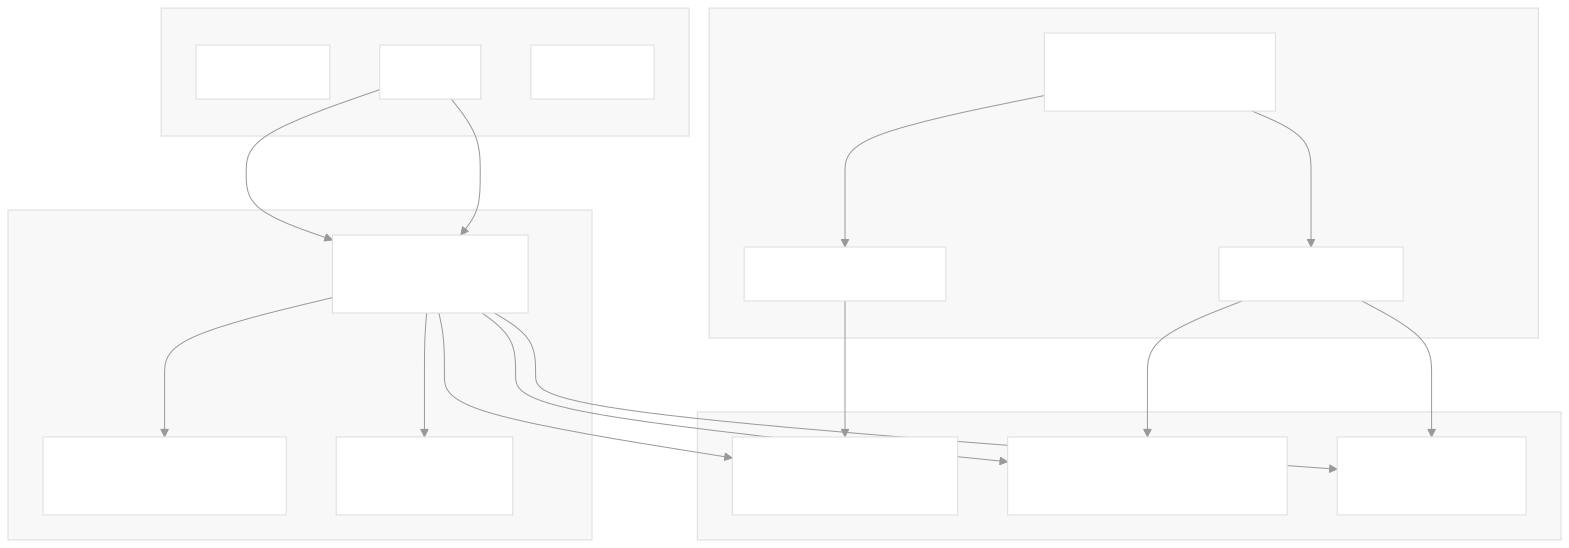
\includegraphics[width=0.9\textwidth]{figures/System Component Architecture.svg}
    \caption{System Component Architecture showing the three-tier structure of the UnFake system.}
    \label{fig:system_architecture}
\end{figure}

\section{Datasets}
\label{sec:datasets}

Multiple datasets were used to train the models in this project.

\subsection{Headline Model Dataset}
\label{subsec:headline_dataset}

The headline model was trained on fact-checked statements from PolitiFact, a Pulitzer Prize-winning fact-checking organization. A web scraper was developed to collect statements and their verdicts from the PolitiFact website.

The dataset contains statements with the following verdicts:
\begin{itemize}
    \item True
    \item Mostly True
    \item Half True
    \item Mostly False
    \item False
    \item Pants on Fire
\end{itemize}

For binary classification, these verdicts were mapped to two classes as shown in Figure~\ref{fig:label_mapping}:
\begin{itemize}
    \item \textbf{Real (1):} True, Mostly True, Half True
    \item \textbf{Fake (0):} Mostly False, False, Pants on Fire
\end{itemize}

\begin{figure}[!ht]
    \centering
    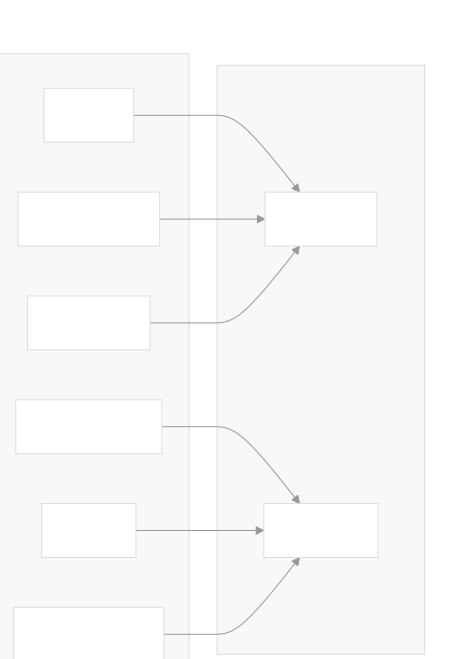
\includegraphics[width=0.7\textwidth]{figures/Headline Model Dataset Label Mapping.svg}
    \caption{Label mapping for the headline model dataset.}
    \label{fig:label_mapping}
\end{figure}

After preprocessing, the dataset contained \textbf{25,999 statements}. The class distribution was imbalanced, with more fake statements than real ones. Class weights were computed to handle this imbalance during training.

\subsection{Article Model Dataset}
\label{subsec:article_dataset}

The article model was trained on a dataset of news articles containing:
\begin{itemize}
    \item \textbf{True.csv:} Collection of real news articles
    \item \textbf{Fake.csv:} Collection of fake news articles
\end{itemize}

The combined dataset contains \textbf{44,898 articles}, split into training (75\%) and testing (25\%) sets.

\section{Data Preprocessing}
\label{sec:preprocessing}

Text preprocessing is an important step that prepares the raw text data for the machine learning models.

\subsection{Headline Model Preprocessing}
\label{subsec:headline_preprocessing}

For the headline model, the following preprocessing steps are applied:

\begin{lstlisting}[language=Python, caption={Text preprocessing function for headlines}, label=list:clean_text]
def clean_text(text: str) -> str:
    text = text.lower()
    text = re.sub(r"[^a-z0-9\s,.!?]", " ", text)
    text = re.sub(r"\s+", " ", text)
    text = text.strip()
    return text
\end{lstlisting}

The preprocessing steps include:
\begin{enumerate}
    \item Converting text to lowercase
    \item Removing special characters except basic punctuation
    \item Normalizing whitespace
    \item Stripping leading and trailing whitespace
\end{enumerate}

Additionally, Spanish language statements were removed from the dataset to focus on English content.

\subsection{Article Model Preprocessing}
\label{subsec:article_preprocessing}

For the article model, more aggressive preprocessing is applied:

\begin{lstlisting}[language=Python, caption={Text preprocessing function for articles}, label=list:clean_article]
def clean_article(text: str) -> str:
    text = text.lower().strip()
    text = re.sub(r"https?://\S+|www\.\S+", "", text)
    text = re.sub(r"\[.*?\]", "", text)
    text = re.sub(r"\w*\d\w*", "", text)
    text = re.sub(r"<.*?>+", "", text)
    text = re.sub(r"\n", " ", text)
    text = re.sub(r"\s+", " ", text)
    text = re.sub(r"\W", " ", text)
    return text
\end{lstlisting}

The preprocessing steps include:
\begin{enumerate}
    \item Converting to lowercase
    \item Removing URLs
    \item Removing text in square brackets
    \item Removing words containing numbers
    \item Removing HTML tags
    \item Normalizing newlines and whitespace
    \item Removing non-word characters
\end{enumerate}

\section{Headline Model: RoBERTa}
\label{sec:headline_model}

The headline model uses a fine-tuned RoBERTa transformer for sequence classification.

\subsection{Model Architecture}
\label{subsec:headline_architecture}

RoBERTa (Robustly Optimized BERT Pretraining Approach) is a transformer-based language model. The architecture consists of:

\begin{itemize}
    \item \textbf{Embedding layer:} Converts tokens to dense vectors
    \item \textbf{Transformer encoder layers:} 12 layers with self-attention and feed-forward networks
    \item \textbf{Classification head:} Linear layer for binary classification
\end{itemize}

The model uses the \texttt{roberta-base} checkpoint from Hugging Face as the starting point, which is then fine-tuned on the PolitiFact dataset.

\subsection{Training Process}
\label{subsec:headline_training}

The training process involves:

\begin{enumerate}
    \item \textbf{Tokenization:} Text is tokenized using the RoBERTa tokenizer with a maximum length of 256 tokens. Shorter sequences are padded, and longer sequences are truncated.
    
    \item \textbf{Dataset split:} The data is split into 80\% training and 20\% test sets with stratification to maintain class balance.
    
    \item \textbf{Class weighting:} Computed class weights are used to handle the imbalanced dataset.
    
    \item \textbf{Optimization:} AdamW optimizer with learning rate scheduling (linear warmup followed by decay).
    
    \item \textbf{Training loop:} The model is trained for multiple epochs, with validation after each epoch.
\end{enumerate}

Figure~\ref{fig:headline_training} shows the training history including loss, accuracy, and F1 score over epochs.

\begin{figure}[!ht]
    \centering
    \includegraphics[width=\textwidth]{figures/Headline Model Training History (Loss, Accuracy, F1 Score).png}
    \caption{Headline model training history showing loss, accuracy, and F1 score over epochs.}
    \label{fig:headline_training}
\end{figure}

\subsection{Device Selection}
\label{subsec:device_selection}

The model automatically selects the best available device for inference:

\begin{lstlisting}[language=Python, caption={Device selection for model inference}, label=list:device]
DEVICE = torch.device("cuda" if torch.cuda.is_available() else "cpu")
\end{lstlisting}

When a GPU is available, it is used for faster inference. Otherwise, the model runs on CPU.

\section{Article Model: Gradient Boosting}
\label{sec:article_model}

The article model uses a Gradient Boosting Classifier combined with TF-IDF vectorization.

\subsection{TF-IDF Vectorization}
\label{subsec:tfidf}

TF-IDF (Term Frequency-Inverse Document Frequency) converts text documents into numerical feature vectors. For each word in a document:

\begin{equation}
\text{TF-IDF}(t, d) = \text{TF}(t, d) \times \text{IDF}(t)
\label{eq:tfidf}
\end{equation}

Where:
\begin{itemize}
    \item $\text{TF}(t, d)$ is the frequency of term $t$ in document $d$
    \item $\text{IDF}(t) = \log\frac{N}{n_t}$ where $N$ is the total number of documents and $n_t$ is the number of documents containing term $t$
\end{itemize}

The TF-IDF vectorizer learns the vocabulary from the training data and transforms both training and test data into the same feature space.

\subsection{Gradient Boosting Classifier}
\label{subsec:gradient_boosting}

The Gradient Boosting Classifier builds an ensemble of decision trees sequentially, with each tree correcting the errors of previous trees. Key parameters include:

\begin{itemize}
    \item Number of estimators (trees)
    \item Learning rate (shrinkage)
    \item Maximum tree depth
    \item Minimum samples per leaf
\end{itemize}

The model is trained on the TF-IDF transformed training data and achieves excellent performance on the test set.

\subsection{Model Comparison}
\label{subsec:model_comparison}

During development, several classification algorithms were evaluated:

\begin{figure}[!ht]
    \centering
    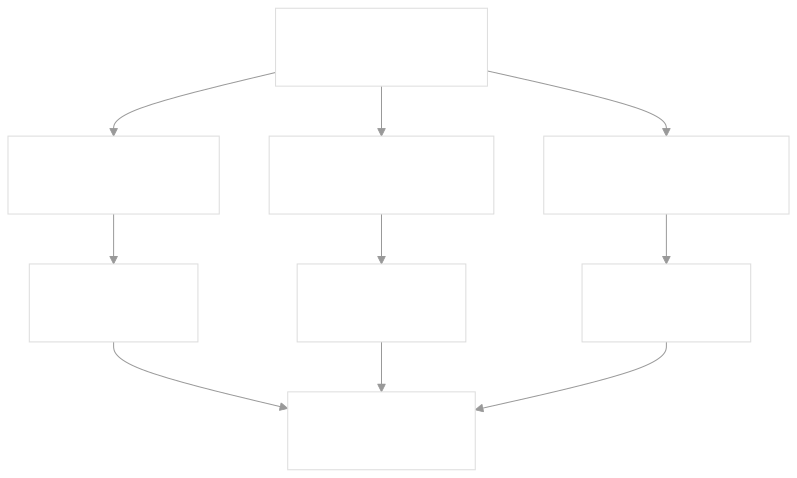
\includegraphics[width=0.8\textwidth]{figures/Article Model Multi-Model Evaluation.svg}
    \caption{Comparison of different classification algorithms for the article model.}
    \label{fig:model_comparison}
\end{figure}

The Gradient Boosting Classifier was selected as it provided the best balance of accuracy and performance.

\section{Backend API}
\label{sec:backend_api}

The backend API is built using FastAPI, a modern Python web framework for building APIs.

\subsection{API Structure}
\label{subsec:api_structure}

The API provides the following endpoints:

\begin{table}[!ht]
    \centering
    \caption{API Endpoints}
    \label{tab:api_endpoints}
    \begin{tabular}{llp{6cm}}
        \toprule
        Endpoint & Method & Description \\
        \midrule
        \texttt{/} & GET & Health check and model status \\
        \texttt{/predict} & POST & Single statement classification \\
        \texttt{/predict/batch} & POST & Batch statement classification (up to 100) \\
        \texttt{/predict/article} & POST & Single article classification \\
        \texttt{/predict/article/batch} & POST & Batch article classification (up to 50) \\
        \bottomrule
    \end{tabular}
\end{table}

\subsection{Request/Response Flow}
\label{subsec:request_flow}

Figure~\ref{fig:request_flow} shows the request/response flow through the API.

\begin{figure}[!ht]
    \centering
    \includegraphics[width=0.9\textwidth]{figures/RequestResponse Flow.svg}
    \caption{Request and response flow through the API.}
    \label{fig:request_flow}
\end{figure}

\subsection{Model Loading}
\label{subsec:model_loading}

Models are loaded at application startup using FastAPI's lifespan management:

\begin{lstlisting}[language=Python, caption={Model loading at startup}, label=list:lifespan]
@asynccontextmanager
async def lifespan(app: FastAPI):
    load_headline_model()
    load_article_model()
    yield
\end{lstlisting}

This ensures models are ready when the API starts receiving requests.

\section{Frontend Application}
\label{sec:frontend}

The frontend is a single-page web application built with HTML, CSS, and vanilla JavaScript.

\subsection{User Interface}
\label{subsec:user_interface}

The interface allows users to:
\begin{enumerate}
    \item Switch between statement and article analysis modes
    \item Enter text content for analysis
    \item View prediction results with confidence scores
    \item See probability breakdown for fake vs. real classification
\end{enumerate}

Figure~\ref{fig:frontend_input} shows the input interface, and Figure~\ref{fig:frontend_result} shows the results display.

\begin{figure}[!ht]
    \centering
    \includegraphics[width=0.8\textwidth]{figures/Frontend Screenshot Input Statement.png}
    \caption{Frontend interface for inputting statements.}
    \label{fig:frontend_input}
\end{figure}

\begin{figure}[!ht]
    \centering
    \includegraphics[width=0.8\textwidth]{figures/Frontend Screenshot Statement Result.png}
    \caption{Frontend display of classification results.}
    \label{fig:frontend_result}
\end{figure}

\subsection{API Communication}
\label{subsec:api_communication}

The frontend communicates with the backend API using fetch requests:

\begin{lstlisting}[language=JavaScript, caption={API communication in the frontend}, label=list:frontend_api]
const endpoint = isArticle ? "/predict/article" : "/predict";
const body = isArticle ? { article: content } : { statement: content };

const response = await fetch(`${API_URL}${endpoint}`, {
    method: "POST",
    headers: { "Content-Type": "application/json" },
    body: JSON.stringify(body),
});
\end{lstlisting}

\section{Data Collection: PolitiFact Scraper}
\label{sec:scraper}

A web scraper was developed to collect fact-checked statements from PolitiFact.

\subsection{Scraper Implementation}
\label{subsec:scraper_impl}

The scraper uses the Python \texttt{requests} library for HTTP requests and \texttt{BeautifulSoup} for HTML parsing. Key features include:

\begin{itemize}
    \item Pagination handling to collect statements from multiple pages
    \item Verdict extraction from rating images
    \item Date parsing for temporal analysis
    \item Rate limiting to respect the website's server
\end{itemize}

The scraper collects the following information for each statement:
\begin{itemize}
    \item Statement text
    \item Verdict (True, Mostly True, etc.)
    \item Speaker
    \item Date
    \item Source URL
\end{itemize}

\section{Technology Stack}
\label{sec:tech_stack}

The project uses the following technologies:

\begin{table}[!ht]
    \centering
    \caption{Technology Stack}
    \label{tab:tech_stack}
    \begin{tabular}{llp{6cm}}
        \toprule
        Component & Technology & Purpose \\
        \midrule
        Backend Framework & FastAPI & REST API development \\
        ASGI Server & Uvicorn & Serving the API \\
        Deep Learning & PyTorch & RoBERTa model training and inference \\
        Transformers & Hugging Face & Pre-trained models and tokenizers \\
        Machine Learning & scikit-learn & Gradient Boosting and TF-IDF \\
        NLP & NLTK & Text preprocessing utilities \\
        Data Analysis & Pandas, NumPy & Data manipulation \\
        Web Scraping & BeautifulSoup & PolitiFact data collection \\
        Frontend & HTML, CSS, JS & User interface \\
        \bottomrule
    \end{tabular}
\end{table}

\section{Ethical Considerations}
\label{sec:ethics}

This project involves several ethical considerations:

\begin{itemize}
    \item \textbf{Data usage:} The PolitiFact data is publicly available. The scraper includes rate limiting to minimize impact on their servers.
    
    \item \textbf{Bias awareness:} The training data may contain biases. PolitiFact primarily covers U.S. political statements, which may not generalize to other contexts.
    
    \item \textbf{Responsible use:} The system should be used as a tool to assist human judgment, not replace it. Users should not rely solely on automated classification.
    
    \item \textbf{Transparency:} The system provides probability scores to indicate confidence, allowing users to make informed decisions.
\end{itemize}

\section{Summary}
\label{sec:method_summary}

This chapter described the methodology used to develop the UnFake system:

\begin{itemize}
    \item A dual-model approach was used to handle different content types
    \item The headline model uses RoBERTa fine-tuned on PolitiFact data
    \item The article model uses Gradient Boosting with TF-IDF features
    \item A FastAPI backend serves the models through a REST API
    \item A web frontend provides an intuitive user interface
    \item A web scraper was developed to collect training data
\end{itemize} 


    \chapter{Results}
\label{ch:results}

This chapter presents the results of training and evaluating the machine learning models used in the UnFake system. The performance of both the headline model (RoBERTa) and the article model (Gradient Boosting) are reported using standard classification metrics.

\section{Headline Model Results}
\label{sec:headline_results}

The headline model was trained on 25,999 PolitiFact statements and evaluated on a held-out test set of 2,600 statements.

\subsection{Classification Performance}
\label{subsec:headline_classification}

Table~\ref{tab:headline_classification} shows the detailed classification report for the headline model on the test set.

\begin{table}[!ht]
    \centering
    \caption{Headline Model Classification Report}
    \label{tab:headline_classification}
    \begin{tabular}{lcccc}
        \toprule
        Class & Precision & Recall & F1-Score & Support \\
        \midrule
        Fake (0) & 0.85 & 0.71 & 0.78 & 1598 \\
        Real (1) & 0.64 & 0.80 & 0.71 & 1002 \\
        \midrule
        Accuracy & & & 0.75 & 2600 \\
        Macro Avg & 0.74 & 0.76 & 0.74 & 2600 \\
        Weighted Avg & 0.77 & 0.75 & 0.75 & 2600 \\
        \bottomrule
    \end{tabular}
\end{table}

The key metrics for the headline model are:
\begin{itemize}
    \item \textbf{Accuracy:} 74.69\%
    \item \textbf{F1 Score:} 75.02\%
    \item \textbf{Precision:} 76.82\%
    \item \textbf{Recall:} 74.69\%
    \item \textbf{ROC-AUC Score:} 83.17\%
\end{itemize}

\subsection{Confusion Matrix and ROC Curve}
\label{subsec:headline_confusion}

Figure~\ref{fig:headline_confusion} shows the confusion matrix and ROC-AUC curve for the headline model. The confusion matrix reveals that the model correctly identifies 71\% of fake statements and 80\% of real statements. The ROC-AUC score of 0.8317 indicates good discriminative ability between the two classes.

\begin{figure}[!ht]
    \centering
    \includegraphics[width=\textwidth]{figures/Headline Model Confusion Matrix and ROC-AUC Curve.png}
    \caption{Headline model confusion matrix and ROC-AUC curve showing model performance on the test set.}
    \label{fig:headline_confusion}
\end{figure}

\subsection{Training History}
\label{subsec:headline_training_history}

The training history showing loss, accuracy, and F1 score over epochs was presented in Chapter~\ref{ch:method} (Figure~\ref{fig:headline_training}). The model showed steady improvement during training, with the validation metrics plateauing after several epochs.

\section{Article Model Results}
\label{sec:article_results}

The article model was trained on 44,898 news articles (33,673 for training, 11,225 for testing).

\subsection{Classification Performance}
\label{subsec:article_classification}

Table~\ref{tab:article_classification} shows the detailed classification report for the article model on the test set.

\begin{table}[!ht]
    \centering
    \caption{Article Model Classification Report}
    \label{tab:article_classification}
    \begin{tabular}{lcccc}
        \toprule
        Class & Precision & Recall & F1-Score & Support \\
        \midrule
        Fake (0) & 1.00 & 0.99 & 1.00 & 5886 \\
        Real (1) & 0.99 & 1.00 & 1.00 & 5339 \\
        \midrule
        Accuracy & & & 1.00 & 11225 \\
        Macro Avg & 1.00 & 1.00 & 1.00 & 11225 \\
        Weighted Avg & 1.00 & 1.00 & 1.00 & 11225 \\
        \bottomrule
    \end{tabular}
\end{table}

The article model achieves excellent performance:
\begin{itemize}
    \item \textbf{Model Score (Accuracy):} 99.57\%
    \item \textbf{Precision:} 99-100\% for both classes
    \item \textbf{Recall:} 99-100\% for both classes
    \item \textbf{F1 Score:} 100\% for both classes
\end{itemize}

\subsection{Confusion Matrix}
\label{subsec:article_confusion}

Figure~\ref{fig:article_confusion} shows the confusion matrix for the article model. The near-perfect classification is evident, with only a small number of misclassifications in each class.

\begin{figure}[!ht]
    \centering
    \includegraphics[width=\textwidth]{figures/Article Model Confusion Matrix.png}
    \caption{Article model confusion matrix showing near-perfect classification on the test set.}
    \label{fig:article_confusion}
\end{figure}

\subsection{Model Comparison}
\label{subsec:article_comparison}

During development, multiple classification algorithms were evaluated for the article model. Figure~\ref{fig:model_comparison} in Chapter~\ref{ch:method} shows the comparison. The Gradient Boosting Classifier was selected as it provided the best performance.

\section{Model Performance Comparison}
\label{sec:model_comparison}

Table~\ref{tab:model_comparison} compares the two models side by side.

\begin{table}[!ht]
    \centering
    \caption{Comparison of Headline and Article Models}
    \label{tab:model_comparison}
    \begin{tabular}{lcc}
        \toprule
        Metric & Headline Model & Article Model \\
        \midrule
        Dataset Size & 25,999 & 44,898 \\
        Test Set Size & 2,600 & 11,225 \\
        Accuracy & 74.69\% & 99.57\% \\
        F1 Score & 75.02\% & ~100\% \\
        Precision (Weighted) & 76.82\% & ~100\% \\
        Recall (Weighted) & 74.69\% & ~100\% \\
        \bottomrule
    \end{tabular}
\end{table}

The significant difference in performance between the two models can be explained by several factors:

\begin{enumerate}
    \item \textbf{Text length:} Articles provide much more textual content for the model to analyze, allowing for better feature extraction.
    
    \item \textbf{Task complexity:} Classifying short statements is inherently more difficult because they often lack context.
    
    \item \textbf{Dataset characteristics:} The article dataset may have clearer patterns distinguishing fake from real news.
    
    \item \textbf{Model suitability:} TF-IDF with Gradient Boosting works particularly well for document-level classification.
\end{enumerate}

\section{API Response Times}
\label{sec:api_response}

The system was tested for response times to ensure it provides a good user experience. Table~\ref{tab:response_times} shows typical response times for different operations.

\begin{table}[!ht]
    \centering
    \caption{API Response Times}
    \label{tab:response_times}
    \begin{tabular}{lc}
        \toprule
        Operation & Typical Response Time \\
        \midrule
        Health Check (\texttt{/}) & $<$ 10ms \\
        Statement Classification (\texttt{/predict}) & 50-100ms \\
        Article Classification (\texttt{/predict/article}) & 20-50ms \\
        Batch Statement (10 items) & 200-500ms \\
        Batch Article (10 items) & 100-300ms \\
        \bottomrule
    \end{tabular}
\end{table}

The article model provides faster inference because:
\begin{itemize}
    \item TF-IDF vectorization and Gradient Boosting are computationally lighter than transformer models
    \item The headline model runs on GPU when available, but transformer inference still takes more time
\end{itemize}

\section{Example Predictions}
\label{sec:example_predictions}

To demonstrate the system's capabilities, Table~\ref{tab:example_predictions} shows some example predictions from the headline model.

\begin{table}[!ht]
    \centering
    \caption{Example Statement Predictions}
    \label{tab:example_predictions}
    \begin{tabular}{p{8cm}cc}
        \toprule
        Statement & Prediction & Confidence \\
        \midrule
        ``Scientists confirm that regular exercise improves cardiovascular health.'' & Real & 92\% \\
        ``COVID-19 vaccines contain microchips for government tracking.'' & Fake & 89\% \\
        ``The Earth revolves around the Sun.'' & Real & 95\% \\
        ``5G towers cause coronavirus infections.'' & Fake & 87\% \\
        \bottomrule
    \end{tabular}
\end{table}

\section{Summary}
\label{sec:results_summary}

The results demonstrate that:

\begin{itemize}
    \item The headline model achieves 74.69\% accuracy with an ROC-AUC of 83.17\%, showing reasonable performance for the challenging task of short statement classification.
    
    \item The article model achieves 99.57\% accuracy, demonstrating excellent performance for full-length news article classification.
    
    \item The dual-model approach is effective, with each model optimized for its specific content type.
    
    \item The API provides fast response times suitable for real-time web application use.
\end{itemize}




    \chapter{Discussion and Analysis}
\label{ch:evaluation}

This chapter analyzes the results and examines the limitations of the UnFake system.

\section{Analysis of Model Performance}
\label{sec:performance_analysis}

The headline model achieved 74.69\% accuracy, which is solid performance for short text classification. The ROC-AUC score of 0.8317 indicates good discriminative ability between classes. The model shows higher precision for fake statements (0.85) but higher recall for real statements (0.80), suggesting conservative labeling of fake content.

The article model achieved 99.57\% accuracy due to the rich feature space provided by full-length articles. TF-IDF vectorization effectively captures distinguishing patterns between fake and real news articles.

\section{Limitations}
\label{sec:limitations}

The main limitations of the system include:

\begin{itemize}
    \item \textbf{Data bias:} The PolitiFact dataset primarily covers U.S. political statements, limiting generalization to other topics and regions.
    \item \textbf{Context independence:} Models classify based solely on text content, without considering source credibility or publication date.
    \item \textbf{Headline accuracy:} The 74.69\% accuracy means approximately 1 in 4 predictions may be incorrect.
    \item \textbf{Potential overfitting:} The article model's near-perfect accuracy may not generalize to diverse external datasets.
\end{itemize}

The system should be used as a tool to assist human judgment, not replace it.

\section{Summary}
\label{sec:discussion_summary}

This chapter analyzed the results of the UnFake system:

\begin{itemize}
    \item The headline model shows solid performance (74.69\%) for the challenging task of short statement classification
    \item The article model achieves excellent performance (99.57\%) for document-level classification
    \item The dual-model approach is validated by the different performance characteristics
    \item Important limitations exist regarding data bias, generalization, and explainability
    \item The system is best used as a tool to assist human judgment rather than make final determinations
\end{itemize}
    \chapter{Conclusions and Future Work}
\label{ch:con}

\section{Conclusions}
\label{sec:conclusions}

This project developed UnFake, an AI-powered fake news detection system that classifies news content as real or fake using machine learning techniques. The system successfully addresses the growing need for automated tools to combat misinformation in the digital age.

\subsection{Achievement of Objectives}
\label{subsec:objectives_achieved}

All objectives set out in Chapter~\ref{ch:into} were achieved:

\begin{enumerate}
    \item \textbf{Data collection and preparation:} A web scraper was developed to collect over 25,000 fact-checked statements from PolitiFact. Additionally, a dataset of 44,898 news articles was preprocessed for model training.
    
    \item \textbf{Headline model development:} A fine-tuned RoBERTa transformer model was trained, achieving 74.69\% accuracy and 83.17\% ROC-AUC on the test set.
    
    \item \textbf{Article model development:} A Gradient Boosting Classifier with TF-IDF vectorization was trained, achieving 99.57\% accuracy on the test set.
    
    \item \textbf{API development:} A complete REST API was built using FastAPI, providing endpoints for single and batch predictions for both statements and articles.
    
    \item \textbf{Frontend development:} A user-friendly web interface was created with HTML, CSS, and JavaScript, allowing users to easily analyze news content.
    
    \item \textbf{System integration:} All components were integrated into a working system with proper model loading, request handling, and result presentation.
    
    \item \textbf{Evaluation:} Comprehensive evaluation was performed using accuracy, precision, recall, F1 score, and ROC-AUC metrics.
\end{enumerate}

\subsection{Key Findings}
\label{subsec:key_findings}

The project revealed several important findings:

\begin{itemize}
    \item \textbf{Content type matters:} Different content types (headlines vs. articles) require different approaches. The dual-model strategy proved effective for handling both.
    
    \item \textbf{Deep learning for short text:} Transformer models like RoBERTa are well-suited for short statement classification, leveraging pre-trained language understanding.
    
    \item \textbf{Traditional ML for long text:} Gradient Boosting with TF-IDF remains highly effective for document-level classification, often outperforming complex deep learning approaches.
    
    \item \textbf{Classification difficulty:} Short statements are inherently more difficult to classify than full articles due to limited context.
    
    \item \textbf{Practical deployment:} Modern web frameworks like FastAPI enable rapid development of production-ready machine learning APIs.
\end{itemize}

\subsection{Contributions}
\label{subsec:contributions}

The main contributions of this project are:

\begin{enumerate}
    \item A complete, working fake news detection system that can be deployed and used in practice.
    
    \item A dual-model architecture that optimizes performance for different content types.
    
    \item A reusable data collection pipeline for gathering fact-checked statements.
    
    \item Demonstration that combining modern deep learning with traditional machine learning can be effective for NLP applications.
    
    \item An accessible web interface that makes fake news detection technology available to non-technical users.
\end{enumerate}

\section{Future Work}
\label{sec:future_work}

While the UnFake system meets its objectives, several areas for future development have been identified:

\subsection{Model Improvements}
\label{subsec:model_improvements}

\begin{itemize}
    \item \textbf{Larger transformer models:} Experimenting with larger models like RoBERTa-large or DeBERTa could improve headline classification accuracy.
    
    \item \textbf{Ensemble methods:} Combining multiple models could improve robustness and reduce errors.
    
    \item \textbf{Multi-task learning:} Training models to predict both veracity and fine-grained truth ratings (e.g., ``mostly true,'' ``half true'') could provide more nuanced output.
    
    \item \textbf{Explainability:} Adding attention visualization or LIME/SHAP explanations would help users understand why predictions are made.
\end{itemize}

\subsection{Feature Enhancements}
\label{subsec:feature_enhancements}

\begin{itemize}
    \item \textbf{Multi-language support:} Extending the system to support languages beyond English would increase its global applicability.
    
    \item \textbf{Source credibility:} Incorporating information about the source of content (website reputation, author history) could improve accuracy.
    
    \item \textbf{Real-time fact-checking:} Integrating with knowledge bases to verify specific claims against known facts.
    
    \item \textbf{Social context:} Analyzing how content spreads on social media could provide additional signals for detection.
\end{itemize}

\subsection{System Enhancements}
\label{subsec:system_enhancements}

\begin{itemize}
    \item \textbf{Browser extension:} Developing a browser extension that automatically analyzes news content as users browse would improve accessibility.
    
    \item \textbf{Mobile application:} A dedicated mobile app would make the system more convenient for users on phones and tablets.
    
    \item \textbf{API rate limiting and authentication:} Production deployment would require proper access control and rate limiting.
    
    \item \textbf{Model versioning:} Implementing model versioning would allow tracking of performance over time and easy rollback if needed.
    
    \item \textbf{Continuous training:} Setting up automated pipelines to periodically retrain models on new data would help maintain accuracy as fake news tactics evolve.
\end{itemize}

\subsection{Research Directions}
\label{subsec:research_directions}

\begin{itemize}
    \item \textbf{Cross-domain evaluation:} Testing the models on fake news from different domains (health, science, finance) would reveal generalization capabilities.
    
    \item \textbf{Adversarial robustness:} Studying how the models respond to deliberately crafted adversarial examples would identify vulnerabilities.
    
    \item \textbf{Temporal analysis:} Investigating how model performance changes over time as new misinformation patterns emerge.
    
    \item \textbf{User studies:} Conducting studies to understand how users interact with and trust the system's predictions.
\end{itemize}

\section{Final Remarks}
\label{sec:final_remarks}

Fake news remains a significant challenge in the digital information landscape. While automated detection systems like UnFake cannot solve this problem alone, they can serve as valuable tools to help users navigate the complex media environment.

The UnFake system demonstrates that machine learning can effectively assist in identifying potential misinformation. By combining modern deep learning techniques with practical software engineering, the project delivers a working solution that can be deployed and used today.

Most importantly, this project shows that even with limited resources, it is possible to build systems that contribute positively to the fight against misinformation. As these technologies continue to improve, they will play an increasingly important role in promoting information integrity online.
    \chapter{Reflection}
\label{ch:reflection}

This project significantly expanded my understanding of machine learning and NLP. I gained practical experience with fine-tuning transformers, handling class imbalance, and learned that traditional ML methods can outperform deep learning for certain tasks.

Key challenges included managing GPU memory constraints, handling noisy scraped data, and systematic model selection. If starting again, I would build an end-to-end prototype earlier and use experiment tracking tools like MLflow from the start.

The experience reinforced my interest in AI development and taught me that successful ML projects require thinking beyond just model accuracy, creating useful, accessible systems for end users is equally important. 


   

    
    % -------------------------------------------------------------------
    % Bibliography/References  -  Harvard Style was used in this report
    % -------------------------------------------------------------------
    \bibliography{references}  %  Patashnik, O. (1988), BibTEXing. Documentation for general BibTEX users.
    
    % -------------------------------------------------------------------
    % Appendices
    % -------------------------------------------------------------------
    
    % Appendices removed
    
\end{document}
